\section{Case study}\label{sec:caseStudy}
In this section we show the application of the proposed UML bridge to a non-trivial case study based on the SysML profile.
SysML is a general-purpose modeling language for systems engineering applications \cite{sysml}, it has been proposed by the OMG group
and supports the specification of  hardware, software, processes, and facilities of a system.
The objective of this case study is to present how each aspect of the proposed approach works in practice on SysML models.
As shown in Figure \ref{fig:caseStudy}, we organized the case study as a seven-steps process:
%
\begin{enumerate}
	\item transformation of the SysML profile into a MOF metamodel called $MM_{sysml}$;
	\item automatic generation of the model transformation that creates MOF-based models from SysML-profiled models;
	\item creation of an annotation model $am_{sysml}$ to slice $MM_{sysml}$;
	\item execution of \textit{MMslicer} and \textit{Tslicer} according to the $am_{sysml}$;
	\item design of a SysML-profiled UML model ($HSUV.uml$ in figure);
	\item transformation of $HSUV.uml$ into its MOF-based counterpart ($HSUV.xmi$);
	\item development of a simple manipulation tool that works on $HSUV.xmi$.
\end{enumerate}
%
\vspace{-.4cm}
\begin{figure}[htbp]
	\centering
		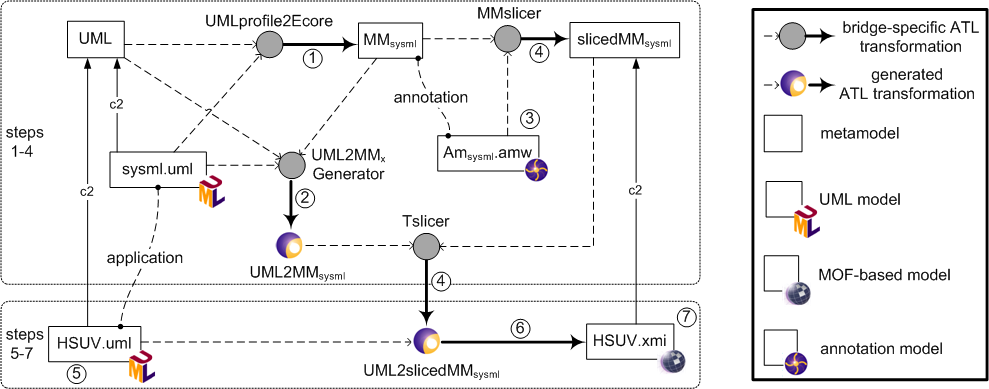
\includegraphics[width=1\textwidth]{figures/caseStudy.png}
	\caption{Overview of the HSUV case study}
	\label{fig:caseStudy}
\end{figure}
\vspace{-.4cm}

%
Before going into the details of each step, it is important to note that steps 1-4 are executed only once, 
then the generated ATL transformation can be re-used every time a SysML model has to be bridged.
Due to space limitations, in this section we will focus more on artifacts at the modeling level, by emphasizing
how designers could benefit from the proposed bridge.
In this case study we use the Papyrus UML tool\footnote{Papyrus UML web site: \small{\url{http://www.papyrusuml.org}}} for
creating the involved UML models. 
%We chose it for two main reasons: 
%(i) a SysML add-in provides support for modeling SysML-like models in Papyrus according to the official SysML specification, and 
%(ii) it is based on Eclipse, so our bridge and the Papyrus tool coexist in the same modeling environment.

\textbf{Step 1.} We firstly consider the SysML profile definition made available by the Papyrus add-in,
and then we transform it into the corresponding MOF metamodel
by means of the $UMLprofile2MOF$ transformation (it is described in Section \ref{sec:metamodelLevel}). 
The resulting $MM_{sysml}$ metamodel is composed of 322 metaclasses (246 from the UML metamodel), 
122 attributes and 665 references (either associations or aggregations).

\textbf{Step 2.} In this step we execute the HOT called $UML2MM_xGenerator$ in order to obtain the
model transformation that takes as input SysML-profiled models and returns MOF-based models. The generated transformation 
($UML2MM_{sysml}$ in figure) is composed of 292 transformation rules, 3625 feature bindings, 10 helpers; the total size of the transformation is 5680 lines of ATL code.

\textbf{Step 3.} In order to slice the obtained $MM_{sysml}$ metamodel and the $UML2MM_{sysml}$ transformation, 
we (automatically) generate an annotation model by means of the second generation mechanism
(see Section \ref{sec:slicing}) by assuming that only UML class diagrams and component diagrams are used.
The generated annotation model ($am_{sysml}$ in figure) contains 37 links to UML metaclasses like Class, Dependency, Interface and so on.
It is important to note that $am_{sysml}$ contains links to only concrete metaclasses in the lower part of the generalization hierarchy, the complete generalization hierarchy is automatically computed by the slicing algorithm presented in Section \ref{sec:slicing}.

\textbf{Step 4.} The newly created annotation model drives the execution of \textit{MMslicer} and \textit{Tslicer}.
They adapt $MM_{sysml}$ and $UML2MM_{sysml}$ by leaving out those concepts that do not
belong either to class or component diagrams. 
The newly adapted metamodel ($slicedMM_{sysml}$) contains 171 metaclasses, 80 attributes and 460 references. 
The size of the adapted transformation ($UML2slicedMM_{sysml}$) is 2690 lines 
of ATL code; it contains 139 transformation rules, 1721 feature bindings and 10 helpers. 
%The $UML2slicedMM_{sysml}$ transformation will be used to transform the initial UML model described in the next step into its 
%corresponding MOF-based model.

\textbf{Step 5.} In order to impartially test the bridge, in this case study we consider the example model provided in the SysML official specification.
This model represents a Hybrid gas/electric powered Sport Utility Vehicle (HSUV) by focussing on its requirements, performance, structure, and behavior. 
Figure \ref{fig:hsuvUML} shows a fragment of SysML diagram in which low-level requirements
(e.g., \textit{RegenerativeBraking})
are derived from system requirements (e.g., \textit{Braking}). 
%Due to space limitations, we do not provide the details of the HSUV model, interested readers can download the full HSUV model from the web page of our bridge. 
%
\vspace{-.4cm}
\begin{figure}
  \centering
  \subfloat[]{\label{fig:hsuvUML}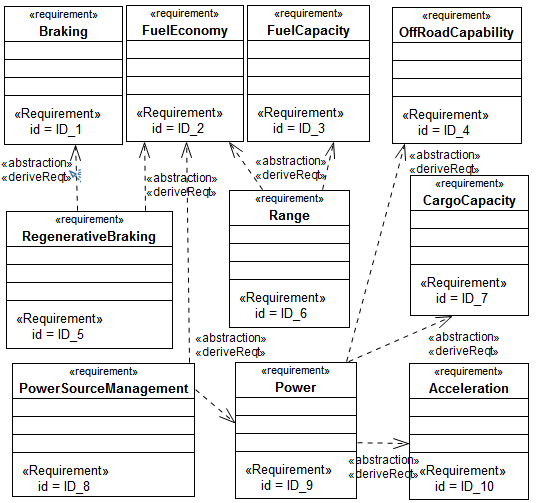
\includegraphics[scale=0.37]{figures/hsuvUML.png}}
 \hspace{2mm}
  \subfloat[]{\label{fig:hsuvMOF}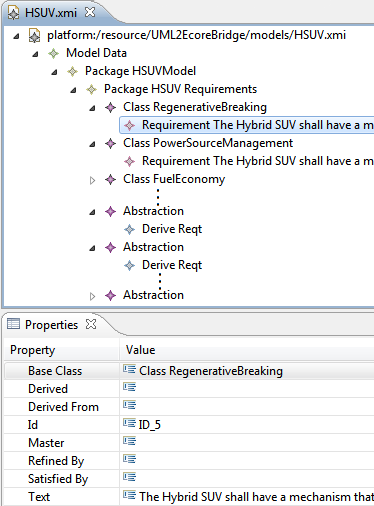
\includegraphics[scale=0.43]{figures/hsuvMOF.png}}
  \caption{HSUV system: a UML model (a) and its corresponding MOF-based model (b)}
  \label{fig:hsuv}
\end{figure}
\vspace{-.4cm}

\textbf{Step 6.} At this point we can execute the $UML2slicedMM_{sysml}$ transformation in order to obtain a MOF-based representation
of the HSUV model. Figure \ref{fig:hsuvMOF} shows a fragment of the obtained model. 
Essentially, it contains the same elements of the source UML model, but (i) each stereotype application (e.g., \textit{Requirement}
was applied to the \textit{Brake} UML class)
has been transformed into an instance of the metaclass corresponding to the applied stereotype,
and (ii) tagged values (e.g., \textit{text} or \textit{id} of \textit{Requirement}) 
have been translated to standard MOF properties. These two differences will facilitate
the manipulation of the HSUV model because stereotypes and tagged values can be accessed as standard MOF elements.

\textbf{Step 7.} In this step we provide a simplified manipulation tool that operates on bridge MOF models. 
Technical details and accuracy are not in the focus of this step of the case study, 
its main goal is to show as clearly as possible how manipulation tools may benefit from our UML bridge. 
The manipulation tool is implemented as an ATL transformation checking if a SysML model follows a simple naming convention.
Listing \ref{lst:manipulationTool} shows an excerpt of this transformation.
It takes as input a SysML model and checks if the identifier of each Requirement starts with the string "ID\_" (line 3);
the transformation generates a Problem element for each requirement that does not follow the convention (lines 10 to 15 in the listing).
%
\begin{lstlisting}[breaklines,style=AMMA,language=ATL,mathescape,rulesepcolor=\color{black},caption=ATL transformation manipulating SysML models,captionpos=b,label={lst:manipulationTool}]
rule checkIDsConvention {
	from
		s : SYSML!Requirement(not s.id.startsWith('ID_'))
--		s : UML2!CLass(
--		  s.isStereotypeApplied(thisModule.requirementStereotype) and 
--			not s.getValue(s.getAppliedStereotypes()->select(e |
--			e = thisModule.requirementStreotype
--		  ).first(), 'id').toString().startsWith('ID_')
--		)		
	to
		t : Problem!Problem (
			severity <- #warning,
			description <- 'the id of ' + s.base_Class.name + ' must start with ID_',
			...
		)
}
\end{lstlisting}

The proposed bridge facilitates
the development of this transformation in different ways, above all: 
(i) the target domain of the transformation (i.e., $slicedMM_{sysml}$) is smaller, 
making the transformation more testable and maintainable, and 
(ii) accessing stereotypes applications and tagged values 
does not require to use UML-specific constructs (lines from 4 to 9 in Listing \ref{lst:manipulationTool} 
show how the condition in line 3 could have been if the input UML model was not bridged with with our approach).

In this case study we showed how the proposed bridge works and how manipulation tools developers benefit
from its application. 
The workflow of the HSUV case study presented in this section can be fully reproduced
since all metamodels, models, and transformations described above are available at the UML bridge web page.
%moreover, since Papyrus UML is open source, also the SysML profile definition can be downloaded.


%The objective of this case study is to present how the UML bridge works at both metamodeling and modeling
%abstraction layers, how the slicing mechanism works in practice, and how a XXX manipulation tool may benefit from
%the application of our approach.